%%%%%%%%%%%%%%%%%%%%%%%%%%%%%%%%%%%%%%%%%
% Journal Article
% LaTeX Template
% Version 1.3 (9/9/13)
%
% This template has been downloaded from:
% http://www.LaTeXTemplates.com
%
% Original author:
% Frits Wenneker (http://www.howtotex.com)
%
% License:
% CC BY-NC-SA 3.0 (http://creativecommons.org/licenses/by-nc-sa/3.0/)
%
%%%%%%%%%%%%%%%%%%%%%%%%%%%%%%%%%%%%%%%%%

%----------------------------------------------------------------------------------------
%	PACKAGES AND OTHER DOCUMENT CONFIGURATIONS
%----------------------------------------------------------------------------------------

\documentclass[12pt,a4paper]{article}
\usepackage[utf8]{inputenc}
\usepackage[francais]{babel}
\usepackage{graphicx} 
\usepackage{amsfonts}
\usepackage{amssymb}
\DeclareGraphicsExtensions{.pdf,.png,.jpg,.mps}

\usepackage{lipsum} % Package to generate dummy text throughout this template
\usepackage[sc]{mathpazo} % Use the Palatino font
\usepackage[T1]{fontenc} % Use 8-bit encoding that has 256 glyphs
\linespread{1.05} % Line spacing - Palatino needs more space between lines
\usepackage{microtype} % Slightly tweak font spacing for aesthetics

\usepackage[hmarginratio=1:1,top=32mm,columnsep=20pt]{geometry} % Document margins
\usepackage{multicol} % Used for the two-column layout of the document
\usepackage[hang, small,labelfont=bf,up,textfont=it,up]{caption} % Custom captions under/above floats in tables or figures
\usepackage{booktabs} % Horizontal rules in tables
\usepackage{float} % Required for tables and figures in the multi-column environment - they need to be placed in specific locations with the [H] (e.g. \begin{table}[H])
\usepackage{hyperref} % For hyperlinks in the PDF

\usepackage{lettrine} % The lettrine is the first enlarged letter at the beginning of the text
\usepackage{paralist} % Used for the compactitem environment which makes bullet points with less space between them

\usepackage{abstract} % Allows abstract customization
\renewcommand{\abstractnamefont}{\normalfont\bfseries} % Set the "Abstract" text to bold
\renewcommand{\abstracttextfont}{\normalfont\small\itshape} % Set the abstract itself to small italic text

\usepackage{titlesec} % Allows customization of titles
\renewcommand\thesection{\Roman{section}} % Roman numerals for the sections
\renewcommand\thesubsection{\Roman{subsection}} % Roman numerals for subsections
\titleformat{\section}[block]{\large\scshape\centering}{\thesection.}{1em}{} % Change the look of the section titles
%\titleformat{\subsection}[block]{\large}{\thesubsection.}{1em}{} % Change the look of the section titles

\usepackage{fancyhdr} % Headers and footers
\pagestyle{fancy} % All pages have headers and footers
\fancyhead{} % Blank out the default header
\fancyfoot{} % Blank out the default footer
\fancyhead[C]{Initiation à l'Arduino $\bullet$ 2016-2017 $\bullet$ BoilingBrains} % Custom header text
\fancyfoot[RO,LE]{\thepage} % Custom footer text

%----------------------------------------------------------------------------------------


%----------------------------------------------------------------------------------------


\begin{document}

%	TITLE SECTION
%----------------------------------------------------------------------------------------
\begin{titlepage}
\title{\vspace{-15mm}\fontsize{42pt}{10pt}\selectfont\textbf{Initiation à l'Arduino}} % Article title

\author{
\large
\normalsize Youtube :\href{https://www.youtube.com/user/M0nsterPr0d}{ BoilingBrains }
\\
\normalsize Twitter :  \href{https://twitter.com/Boiling_Brains_}{ @Boiling\_Brains\_ }
\\
\normalsize Facebook :  \href{https://www.facebook.com/Boiling-Brains-995101330555512/?fref=ts}{Boiling Brains} 
\\
\normalsize \href{mailto:monsterprod01@gmail.com}{monsterprod01@gmail.com} % Your email address
\vspace{-5mm}
}
\date{}


\begin{figure}
    \centering
    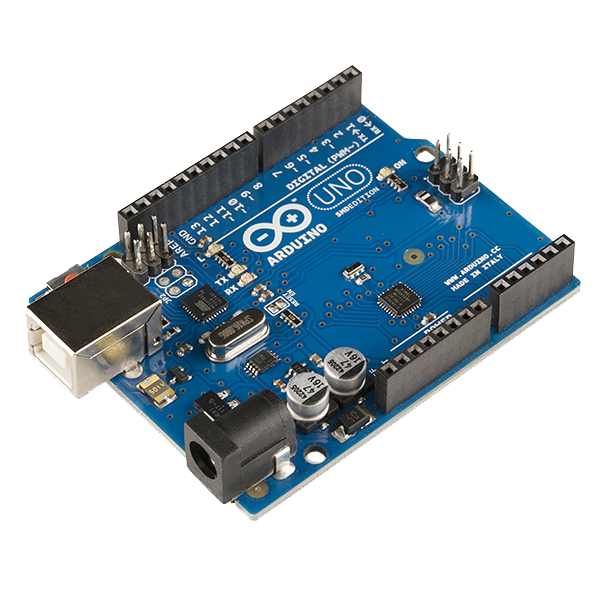
\includegraphics[scale=1.7]{pagegarde.png}
\end{figure}

\end{titlepage}

\maketitle % Insert title

\renewcommand*\contentsname{Sommaire}




\thispagestyle{fancy} % All pages have headers and footers

%----------------------------------------------------------------------------------------
%	ARTICLE CONTENTS
%----------------------------------------------------------------------------------------
\newpage
\tableofcontents
\newpage 

\section*{\LARGE Introduction}

\bigskip
Ce document est une reprise des vidéos “initiation à l’Arduino” réalisées sur la chaîne Youtube \textbf{BoilingBrains}. Il s’agit du format texte des vidéos si vous préférez ( même si c’est un peu bizarre à dire).

\bigskip

Nous tenons à signaler que les personnes ayant vu les trois vidéos en questions, n’apprendrons pratiquement rien de nouveau ici, hormis quelques compléments.

\subsubsection*{Quel est le but de ce document ?}

Réunir les trois vidéos pour proposer un "recueil" permettant de débuter en Arduino et grâce auquel chacun pourra avancer à son propre rythme. C'est différent du format vidéo où on se sent un peu obligé de finir un épisode avant de s'arrêter.
\\
\\
\textbf{Avant de vous laissez démarrer, nous souhaitons préciser que ce document pourrait contenir l'une ou l'autre erreur. N'hésitez donc pas à nous le signaler si vous remarquez quelque chose de "suspect".}
\\
\\
Ce recueil est composé de 3 grandes sections : 
\begin{compactitem}
\bigskip
\item Hardware
\item Software
\item Programmation
\end{compactitem}
\bigskip
Après ces 3 sections, vous serez capable de faire tout ce que vous voudrez avec l’Arduino (ou pas). Je vous rappelle que le but de ce document est de vous aider à vous lancer et non de faire de vous des experts dans le domaine. Après, comme avec tout, il faudra bien évidemment de la pratique avant de pouvoir faire de grandes choses mais c’est en forgeant qu’on devient forgeron ( n’est-ce pas ?).
\\
\\
Bref, commençons !

\newpage
\section{\LARGE Hardware}
Nous avons commencé la série Arduino en présentant des composants tel que la LED, le bouton poussoir, la photorésistance,... dans le but d’introduire de futurs projets qui arriveront sur la chaîne. Mais avant d’aller plus loin, il serait intéressant de revenir sur les bases même de l’Arduino.

\subsection{\textit{\textbf{Qu’est ce que l’Arduino ?}}}
\
L’Arduino est une carte programmable (circuit imprimé)  qui permet de faire de l'électronique de manière très simple. En effet, elle possède une structure ergonomique (les entrées et sorties sont bien alignées et indiquées). La programmation qui s’en suit est simplifiée et les mêmes commandes reviennent souvent. C’est donc le meilleur moyen d’apprendre l’électronique en partant de 0 et de faire du prototypage ou du développement. Cette carte est “open source”, ce qui signifie que vous avez par exemple accès aux plans de la carte.
\\
\\
Il existe différents types d’Arduino et à chaque types correspond une forme et une taille différente.
Nous n’allons pas tous les citer mais nous avons par exemple : 
\begin{compactitem}

\item L'Arduino UNO (la version que nous utilisons actuellement pour nos vidéos) 
\\
\item L’Arduino MEGA qui possède plus d’entrées et de sorties ainsi qu'une mémoire plus conséquante.
\\
\item L’Arduino Nano qui comme son nom l’indique est beaucoup plus petite que ses homologues.
\end{compactitem}



\subsection{\textit{\textbf{De quoi est composée cette bestiole?}}}
1. Alimentation
\\
\\
La carte Arduino peut être alimentée de deux façons : soit par le port USB relié à l’ordinateur, soit avec  un transformateur secteur de tension adéquate via la prise jack ( on peut également utiliser des piles).
\\
\\
L’Arduino accepte des tensions continues de 6 à 20V mais il est conseillé de ne pas dépasser les 12V. La marge de sécurité offre une protection contre les éventuels creux de tension indésirables. La carte est dotée d’un régulateur de tension qui va ramener la tension d’alimentation à  5V et la garder constante au cas où on alimente avec une tension supérieure. De toute manière, en alimentant l’Arduino au port USB de l’ordinateur on est sûr d’avoir une tension de 5V.
\\
2. Microcontrôleur
\\
\\
Le microcontrôleur est l'élément le plus important de la carte Arduino.
 Un microcontrôleur est un circuit intégré (IC) qui rassemble les éléments essentiels d’un ordinateur : processeur (CPU), mémoires, horloge interne et ports d’entrées et de sorties (I/O).
 \\
 Le rôle du CPU est d'exécuter des programmes stockés en mémoire.
\\
Il y a 3 types de mémoire dans un Arduino :
\\
\begin{compactitem}

\item La mémoire FLASH : Cette mémoire sert à stocker les programmes à exécuter par le CPU. C’est une mémoire non volatile , ce qui signifie que les données sont conservées même lorsqu’on coupe l’alimentation. L’Atmega 328 en possède 32 Ko.
\\
\item La mémoire SRAM ( Static Random Access Memory) : Cette mémoire permet de stocker des données temporaires tel que les variables de notre programme. Contrairement à la mémoire FLASH, la SRAM est une mémoire volatile. Elle est très rapide et l’Arduino UNO en possède seulement 2 Ko. On peut comparer cette mémoire à la RAM d’un ordinateur.
\\
\item La mémoire EEPROM (Electrically Erasable Programmable Read Only Memory ou mémoire morte effaçable électriquement et programmable) : Elle permet le stockage de données persistantes ( données de log ou états devant être conservés). C’est une mémoire lente mais non volatile. L’Arduino UNO possède 1Ko de cette mémoire. C’est le “disque dur” de notre carte.
\\
\end{compactitem}
\
L’horloge interne (ou oscillateur) permet de cadencer (rythmer) les actions du CPU car ce dernier ne travaille pas en continue, il exécute un certain nombre de calculs par seconde.


[\textit{La puissance de calcul d'un processeur est exprimée en Hertz. Aujourd'hui les processeurs sont capables d'atteindre plus de 2Ghz (Giga Hertz = Milliards de Hertz) soit plusieurs milliards de calculs par seconde.}]  
\\
\\
Les ports d’entrées et de sorties sont des connexions qui relient le microcontrôleur au monde extérieur. C’est l’interface entre le composant électronique et le monde réel. On peut raccorder divers composant à cette interface : LED, photorésistance, bouton-poussoir, … Si on retourne l’Arduino, on remarque qu’un certain nombre d’entrées/sorties sont reliées aux pattes du microcontrôleur. C’est notre fameuse interface avec le monde réel. Lorsqu’on branche des fils dans ces entrées/sorties, c’est comme si on les connectait directement aux pattes du microcontrôleur.
\\
\\
Les microcontrôleurs permettent de diminuer la taille, la consommation électrique et le coût des produits.
On les utilise dans les systèmes embarqués comme les contrôleurs des moteurs automobiles, les télécommandes, l’électroménager, les jouets, la téléphonie mobile,... les applications sont très nombreuses.
\\
\\
En bref, les microcontrôleurs perçoivent des influences extérieures par l’intermédiaire de capteurs, traitent les données puis envoient des ordres de commandes vers l’extérieur. C’est en quelque sorte le cerveau de l’Arduino.
\\
\\
\\
3. Broches ou Pins
\\
\\
Les pins ou entrées/sorties de la carte Arduino sont principalement :
\begin{compactitem}

\item Soit des connexions d’alimentation (5V/3.3V/Vin/Ground). C’est par là que sont alimentés les circuits qu’on réalise.
\\
\item Soit des entrées/sorties digitales ou analogiques. Nous verrons plus de détails concernant cela dans la section Software.

\end{compactitem}
\bigskip
\begin{figure}[h!]
    \centering
    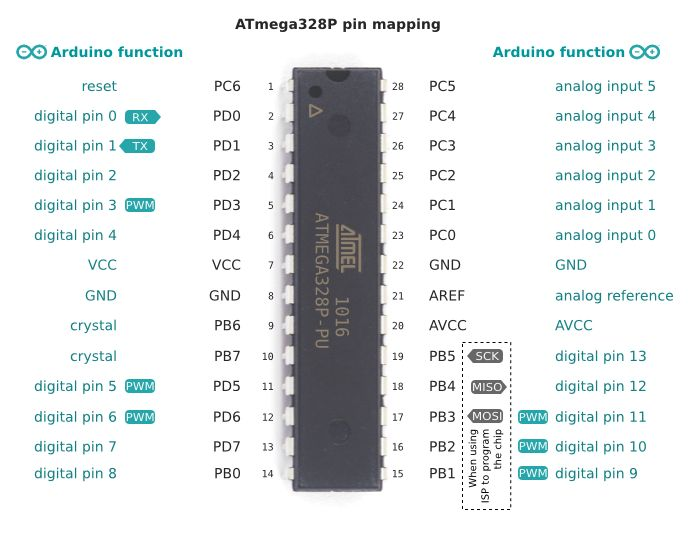
\includegraphics[scale=0.5]{PINMAP.jpg}
    \caption{Broches du microcontrôleur ATmega328P}
    \label{fig:my_label}
\end{figure}


\newpage
\begin{figure}[h!]
    \centering
    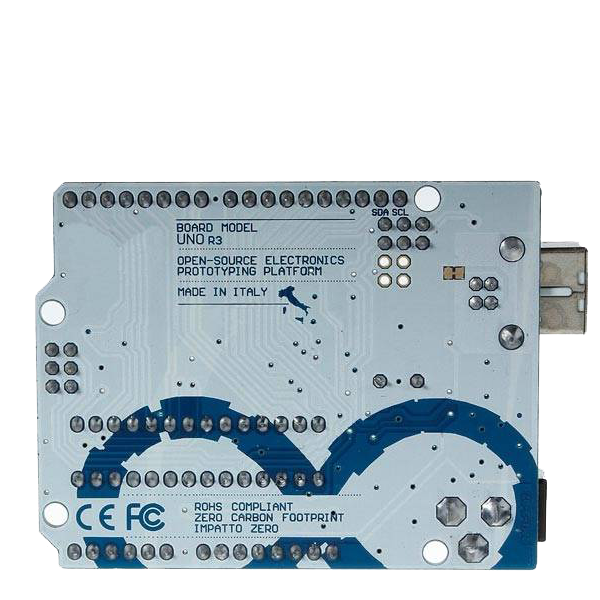
\includegraphics[scale=0.45]{facearriere2.png}
    \caption{Face arrière de la carte Arduino UNO}
    \label{fig:my_label}
\end{figure}


4. Bouton Reset
\\
\\
Le bouton Reset présent sur la carte, permet de tout réinitialiser et donc également effacer le programme en mémoire.
\\
\\
\\
5. LED d'alimentation
\\
\\
La LED d’alimentation est une LED témoin qui clignote lorsque la carte Arduino est alimentée.

%------------------------------------------------
\subsection{\textit{\textbf{Matériel nécessaire}}}
Pour vous lancer, mis à part la carte Arduino, il vous faudra encore ce qu’on appelle une “planche à pain” ou breadboard ( en anglais, c’est toujours plus stylé). Une breadboard est une plaque d’essai sans soudure. C’est le support sur lequel on réalise les montages.

\begin{figure}[h!]
    \centering
    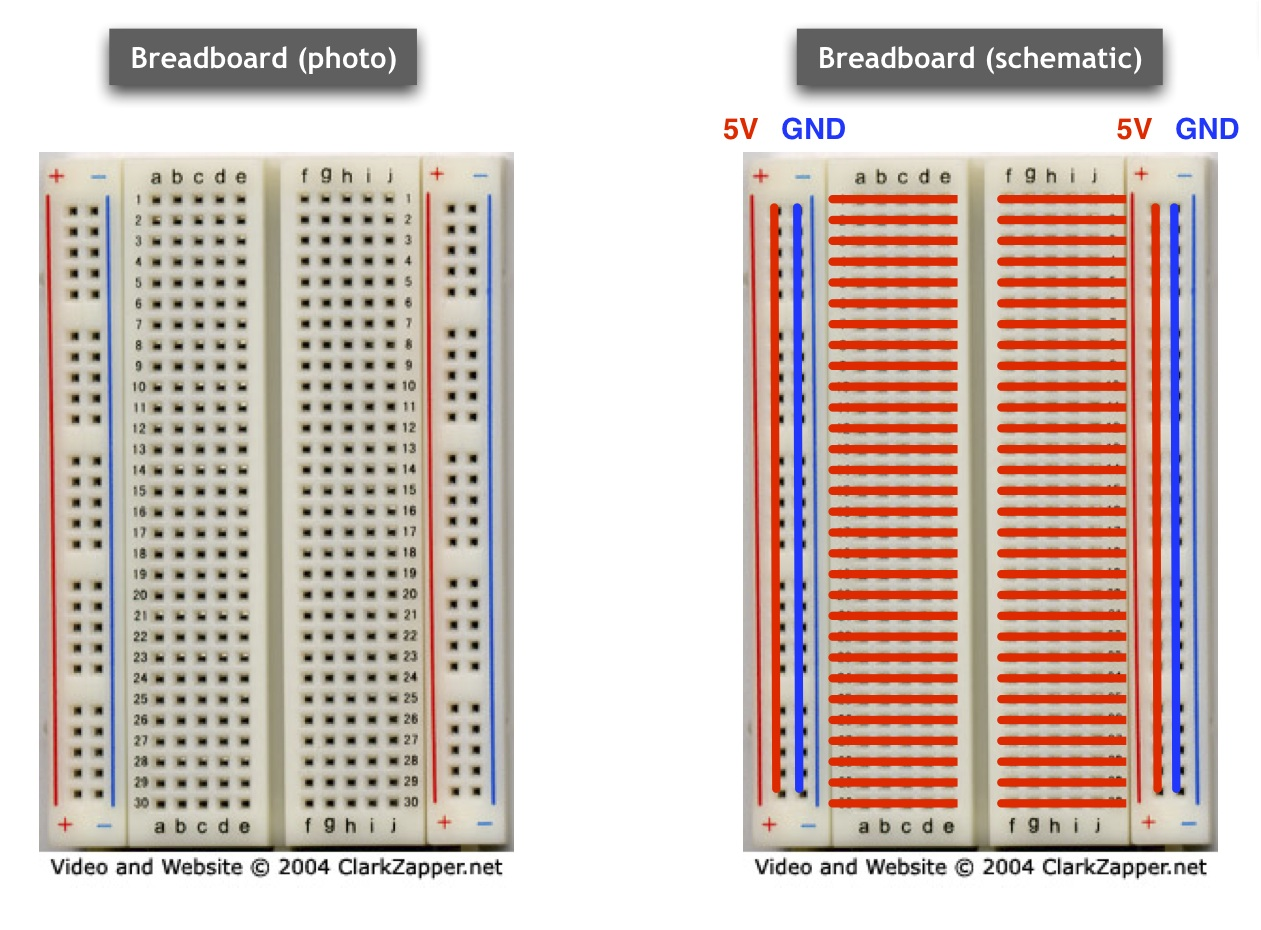
\includegraphics[scale=0.49]{breadboard.jpg}
    \caption{Illustration des connections dans une breadboard}
    \label{fig:my_label}
\end{figure}
\bigskip
Il faudra donc faire aucune soudure. Il suffira d'insérer les composants et câbles dans les petits trous qui sont des contact métallique à ressort. 

\newpage
La figure ci-dessus, montre la manière dont les différents contacts sont électriquement reliés entre eux. 
\\
\\
Un circuit assemblé sur une telle plaque ne sera bien évidemment pas aussi solide qu’un circuit imprimé mais ce n’est pas très important vu qu’on utilisera ça uniquement pour expérimenter des montages provisoires.
\\
\\
Maintenant que vous avez votre carte Arduino ainsi que votre breadboard, il vous faudra des composants et quelques câbles pour réaliser vos montages. Il faut savoir que niveau composants, vous avez largement le choix.
En effet, il existe vraiment beaucoup de composants compatibles avec l’Arduino :
leds,moteur, capteur de température, ecran lcd, module wifi, …. il y a vraiment de TOUT !
\\
\\
Vous vous demandez ce qu’il est possible de faire avec un Arduino, j’aimerais dire TOUT, tellement les applications sont nombreuses. Vous pouvez vraiment réaliser un peu ce que vous voulez avec un Arduino (sans blague).La seule vraie limite c’est votre imagination.
\\
\newpage
\section{\LARGE Software}
\subsection{\textit{\textbf{Logiciel Arduino}}}
La carte Arduino se programme à l’aide d’un environnement de développement spécialement créé pour Arduino. Ce logiciel est plus facile à prendre en main et plus intuitif que les logiciels classiques de programmation.
En plus, il ne faut même pas l’installer. Il suffit de décompresser l’archive et de lancer le logiciel. Vous pouvez le télécharger gratuitement sur :


\begin{center}
\url{http://arduino.cc/en/Main/Software}
\end{center}

\bigskip
Si on ouvre le logiciel, on tombe sur cette interface : 

\begin{figure}[h!]
    \centering
    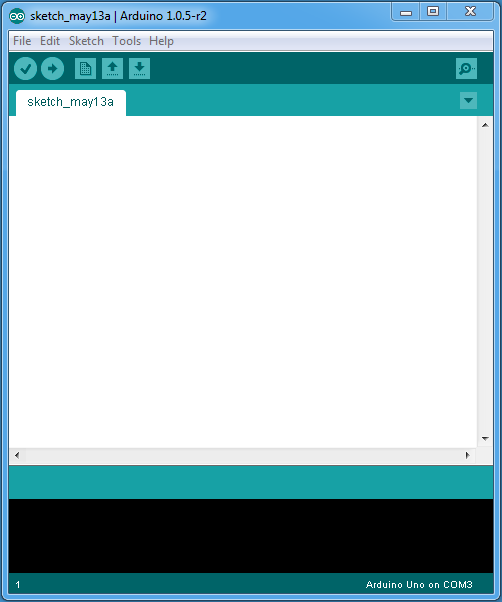
\includegraphics[scale=0.7]{sketchVide.png}
    \caption{Interface du logiciel}
    \label{fig:my_label}
\end{figure}

Si aucun programme n’a été chargé, le croquis (sketch) porte un nom par défaut :
"sketch\_mois+date+x"


\begin{compactitem}
    \item[•] date  = jour du mois
    \item[•] x     = une lettre de l'alphabet $\rightarrow$ si c’est le premier sketch
    de la journée qu’on ouvre, ça sera \textbf{a}, si c’est le deuxième alors \textbf{b},....
\end{compactitem}

\newpage
Mais tout ça c’est du détail … Intéressons nous aux différents boutons.

\bigskip
\begin{figure}[h!]
    \centering
    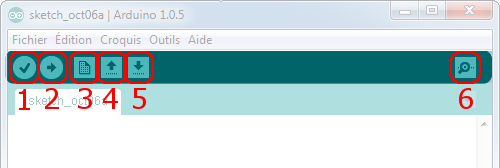
\includegraphics[scale=1]{boutons.png}
    \caption{Boutons de l'interface}
    \label{fig:my_label}
\end{figure}

\bigskip
Nous avons : 

\begin{itemize}
    \item[1.] \textit{\underline{\textbf{Vérifier}}} : Vérifie et compile ( compiler = transformer un programme écrit en  language de programmation en language machine $\rightarrow$ binaire) le programme qu’on a écrit. Si jamais il y’a des erreurs dans notre code, elles seront affichées dans la fenêtre noire en bas.
    
    \bigskip
    \item[2.] \textit{\underline{\textbf{Téléverser}}} : compile le programme et l’envoi sur la carte Arduino.
    
    \bigskip
    \item[3.] \textit{\underline{\textbf{Nouveau}}} : Ouvre un nouveau croquis
    
    \bigskip
    \item[4.] \textit{\underline{\textbf{Ouvrir}}} :  Permet d’ouvrir un croquis déjà existant
    
    \bigskip
    \item[5.] \textit{\underline{\textbf{Sauvegarder}}} : Enregistre le croquis en cours
    
    \bigskip
    \item[6.] \textit{\underline{\textbf{Moniteur série}}} : Ouvre ce qu’on appelle le moniteur série, qui est une fenêtre qui permet de voir des données échangées entre la carte Arduino et le PC en cours d'exécution d’un programme. Ça permet de voir la valeur des capteurs utilisés dans le montage. (son utilisation n’est pas obligatoire). 
\end{itemize}

\newpage
\subsection{\textit{\textbf{Communication avec la carte}}}
Avant de relier l’Arduino au PC par câble USB, il faut choisi le modèle de la carte :

\begin{figure}[h!]
    \centering
    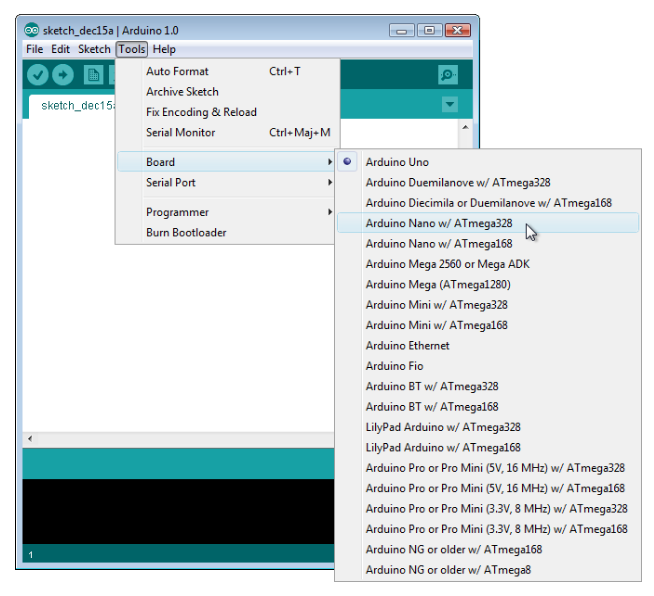
\includegraphics[scale=1.1]{choixcarte.PNG}
    \caption{Choix de la version de notre Arduino}
    \label{fig:my_label}
\end{figure}

\newpage
Après cela, on sélectionne le port COM virtuel utilisé. Normalement cette étape se fait toute seule mais il est conseillé d’aller vérifier si on est sur le bon port à chaque fois qu’on branche l’Arduino, histoire d’éviter des soucis ( carte non détectée).

\bigskip
\begin{figure}[h!]
    \centering
    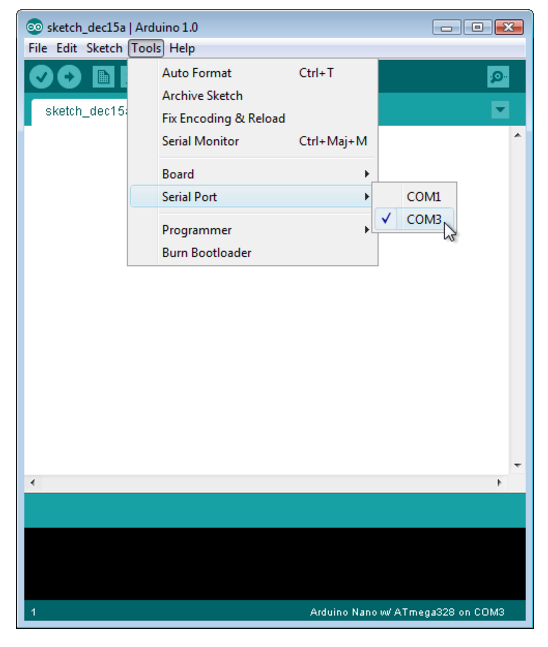
\includegraphics[scale=1.2]{choixport.PNG}
    \caption{Choix du port de communication}
    \label{fig:my_label}
\end{figure}

\newpage

Si vous avez plusieurs cartes Arduino, je vous conseille d’utiliser un port USB différent pour chaque carte ( pas obligé). Après avoir branché notre carte sur l'ordinateur,  nous allons vérifier si la connexion entre l’Arduino et le PC peut s’établir sans problème. 
Pour cela, on charge le programme d’exemple appelé \textit{\textbf{“Blink”}} :

\begin{figure}[h!]
    \centering
    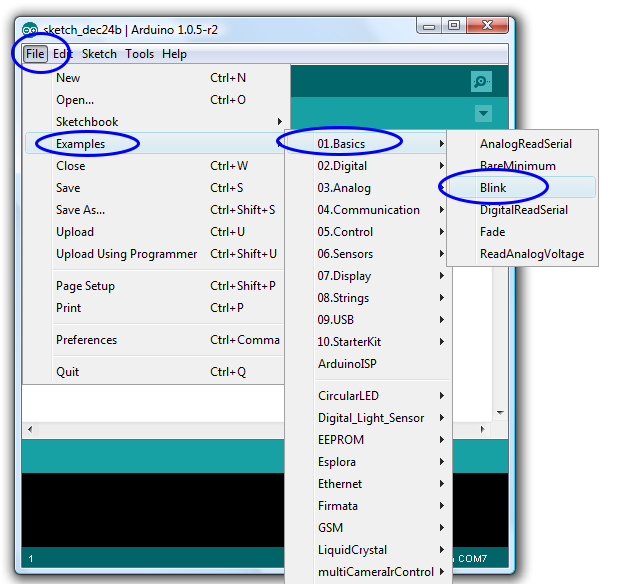
\includegraphics[scale=0.7]{blink.png}
    \caption{Programme d'exemple "Blink"}
    \label{fig:my_label}
\end{figure}

\newpage
Et on téléverse : 
\begin{figure}[h!]
    \centering
    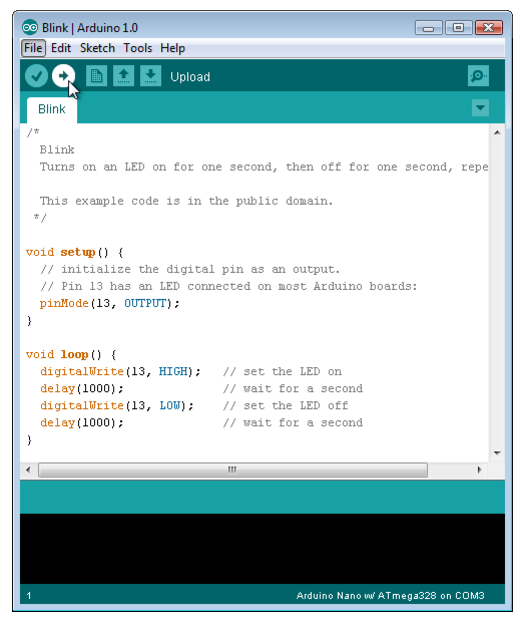
\includegraphics[scale=0.9]{televersement.PNG}
    \caption{Téléversement de notre code}
    \label{fig:my_label}
\end{figure}

\bigskip
Si tout se passe bien et qu’on a pas d’erreur, la LED 13 commence à clignoter :+ montrer la LED qui clignote sur la carte

\begin{figure}[h!]
    \centering
    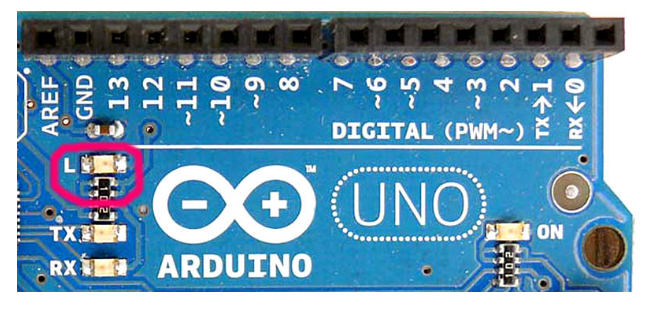
\includegraphics[scale=0.5]{led.PNG}
    \caption{LED 13}
    \label{fig:my_label}
\end{figure}

Nous pouvons donc enfin passer à la partie la plus importante lors d'une session "Arduino". Vous aurez deviné, je parle de la programmtion !

\newpage
\section{\LARGE Programmation}
Il existe plusieurs languages de programmation. Dans le cas de l’Arduino, nous allons programmer dans un language qui se rapproche du C et qui n’as pas vraiment de nom … 
C’est un language qui a été spécialement développé pour l’Arduino….disons que le C classique est un peu trop “cryptique”. Là on aura quelque chose de beaucoup plus simple.

\bigskip
Commençons par la structure générale d’un programme...

\begin{figure}[h!]
    \centering
    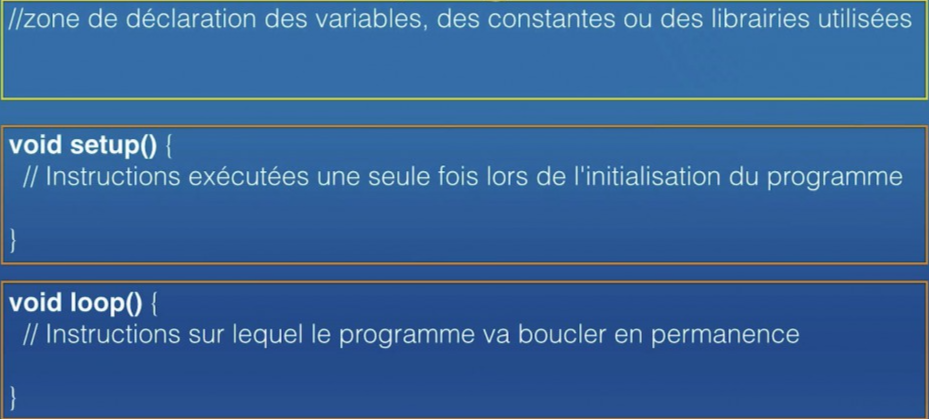
\includegraphics[scale=0.7]{structprog.PNG}
    \caption{Structure d'un programme}
    \label{fig:my_label}
\end{figure}

\subsection{\textit{\textbf{Structure générale d’un programme}}}

Un programme Arduino se structure en trois parties :
la déclaration et l’initialisation des variables, \textit{\textbf{"le setup()"}} et \textit{\textbf{"le loop()"}}

\bigskip

Les variables sont ce qu’il y a de plus important dans un programme. C’est le nom associé à un certain emplacement de la mémoire qui pourra être utilisé pour stocker par exemple, le résultat d’une opération.

\bigskip

La mémoire dont on dispose est en général limitée, il existe donc plusieurs type de variable différentes. Chaque type occupe un certain nombre d’octets ( plus ou moins grand selon le type de la variable).  Le but sera donc d’utiliser le type de variable adaptée, qui optimise la place occupée en mémoire. Dans les petits programmes cela n’as pas vraiment d’importance car on ne dépassera jamais la mémoire maximum disponible sur notre carte. Une variable se déclare de la façon suivante :
\begin{center}
type nom\_de\_la\_variable = valeur; 
\end{center}
Sans qu’une valeur ne lui soit affectée, la variable est initialisée à 0. Après avoir déclarer nos variables, on passe dans le second bloc c-à-d. le setup, qui est ce qu’on appelle une fonction. 

\bigskip

Une fonction est un ensemble d’instructions reunies en une unité logique possèdant un nom évoquateur afin d’être appellée comme une instruction ordinaire. Toutes les instructions qu’elle contient sont éxecutée en un seul bloc.Dans la fonction setup, on va programmer les différentes broches du microcontroleur. Si on branche par exemple un composant sur la broche 8 de la carte, il faut dire si cette broche est utilisée en entrée (INPUT) ou en sortie (OUTPUT).

Dans le cas d’un capteur, la broche devra être déclarée en entrée car le capteur envoie des informations à la carte tandis que dans le cas d’une led qui est un actionneur, on la déclarera en sortie. Le setup servira également a déclarer une connexion série ou une éventuelle connexion bluetooth.

\bigskip
Le dernier bloc est également une fonction nommée loop qui est une boucle infinie…
c’est elle qui contiendra les tâches que doit effectuer notre programme c-à-d. la logique au moyen de laquelle seront interrogés les capteurs 
( exemple : donne moi la température toute les x secondes) et commandé les actionneurs ( exemple : allumer une led ou faire tourner un moteur). Les instructions se trouvant dans cette boucle seront répétées jusqu’à la mise hors tension de la carte Arduino.

\subsection{\textit{\textbf{Fonctions propres à Arduino}}}

Mis à part le setup et le loop, l’Arduino possède un grand nombre de fonctions différentes prête à être utilisées. La particularité de ces fonctions est qu’elles sont de haut niveau c-a-d qu’elles permettent de faire une série de chose plus ou moins “complexes” en un minimum de ligne de code. Ces fonctions masquent la complexité de l’Arduino et rendent la programmation accessible à tous. 

\bigskip
De toute les fonction disponibles sur l’Arduino,seules 5 parmis elles, reviennent assez souvent ( pour pas dire tout le temps ou presque) :

\bigskip
On vous a dit que le setup servait à programmer les différentes broches de notre microcontrôleur. Pour ce faire, on utilise la fonction pinMode (pin,mode) qui permet de définir le sens de fonctionnement de la broche appelée PIN soit en entrée (mode = INPUT) ou en sortie (mode= OUTPUT).

\newpage
Avant de présenter les 4 autres fonctions, il faut savoir que l’Arduino possède deux type de ports : 

\bigskip
\begin{enumerate}
    \item  Des ports \textit{\textbf{analogiques}} qui reçoivent ou envoient des signaux pouvant prendre n’importe quelle valeur au cours du temps comprise entre deux extrema ( =signal analogique)
    \item Des ports  \textit{\textbf{numériques}} qui eux, ne peuvent recevoir ou envoyer que des minimas (0V) et des maximas (5V) et aucune valeur intermédiaire.
\end{enumerate}
   
\bigskip
Maintenant que nous savons ça, nous pouvons présenter dans un premier temps les fonctions associé à un port numérique et ensuite celles associées aux ports analogiques :

\bigskip
\begin{itemize}
   \item[] \textit{\textbf{digitalWrite(pin, value)}}  :  Envoi un niveau bas (0) ou un niveau haut (5V) sur la broche spécifiée.
   \bigskip
   \item[] \textit{\textbf{digitalRead(pin)}} : Lit le niveau de tension (0 ou 5V) de la broche et retourne la valeur
\end{itemize}
\

 [\textit{Il faut savoir que les développeurs ont associé le niveau bas à une constante appelée LOW qui correspond à la valeur 0V et le niveau haut à une constante appelé HIGH qui correspond à 5V et donc dans value, on marquera LOW ou HIGH.}]
 
\bigskip
 
 Concernant les ports analogiques, c’est un peu plus compliqué car le microcontrôleur ne traite que des signaux numériques. Les signaux analogiques devront passer par ce qu’on appelle un convertisseur A/D avant d’être pris en charge par le microcontrôleur. Le convertisseur recevra une tension entre 0 et 5V venant de notre capteur et la transformera en un entier compris entre 0 et 1024.

\subsubsection*{Pourquoi 1024 ?} 
Car à la sortie du convertisseur, nous aurons un nombre binaire écrit sous 10 bits qui est la résolution de notre microcontrôleur et $2^{10}=1024$.

\bigskip
\underline{Petit exemple pour mieux comprendre}: 

\bigskip
Imaginons que nous avons une valeur de tension correspondant à 1V. La première étape va être de convertir cette valeur en un entier compris entre 0 et 1024. 
Dans notre cas, 1V correspond à 205 ( si on arrondi à l’entier le plus proche). La dernière étape consistera à convertir 205 en un nombre binaire de 10 bits c-à-d “00011001101”.

\bigskip
Maintenant que nous avons compris la conversion digitale -> analogique, intéressons-nous aux fonctions associées aux ports analogiques :

\bigskip
\begin{itemize}
   \item[•] \textit{\textbf{analogRead(pin)}}  lit la tension sur une broche analogique et renvoie ensuite la valeur lue sous forme de 10bits comme expliqué précédemment.
   \bigskip
   \item[•] \textit{\textbf{analogWrite(pin, value)}}  génère un train d’impulsion ou ce qu’on appelle un signal PWM ( modulation de la largeur d’impulsion en français).  
\end{itemize}
\bigskip

Un signal PWM est un signal logique ( valant 0 ou 1) à période constante mais dont le rapport cyclique est défini par l’utilisateur. Ce dernier correspond à la durée d’impulsion ( signal à 1) par rapport à cette période fixe.
 
\subsubsection*{Comment s’utilise cette fonction ?}

Il faut tout d’abord être branché sur une broche PWM de la carte. On spécifie ensuite 2 paramètres : le numéro de la broche sur laquelle on est ainsi que le rapport cyclique qui doit être compris entre 0 (0\%) et 255 (100\%). 

\bigskip

\textit{[Pour plus de détails concernant les PWM, nous vous conseillons la vidéo de U = RI} \footnote{\url{https://www.youtube.com/watch?v=CSReyYwbGRY}} \textit{qui explique très bien la chose.}]


\begin{figure}[h!]
    \centering
    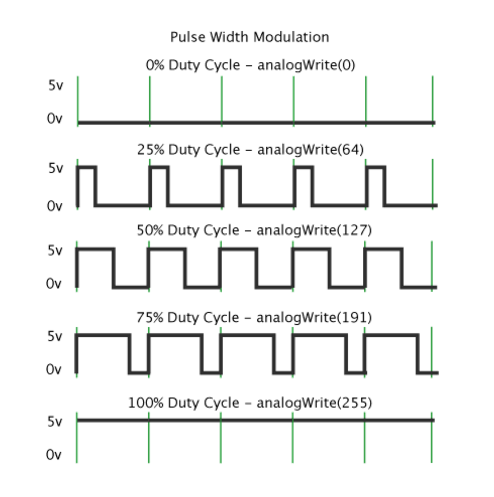
\includegraphics[scale=0.8]{pwm2.PNG}
    \caption{PWM}
    \label{fig:my_label}
\end{figure}


\newpage
Arduino possède des fonctions  concernent la gestion du temps. Voici 3 exemples intéressants : 

\bigskip
\begin{itemize}
    \item[•] \textit{\textbf{delay(ms)}}
\end{itemize}

La fonction delay permet de mettre notre programme en pause pendant la durée (en millisecondes) passée en paramètre. C’est une fonction qu’on utilise dans 99\% des programmes écrit. Elle permettra par exemple de faire clignoter une LED, chose que nous avons faite dans notre toute première vidéo de la série.
\footnote{\url{https://www.youtube.com/watch?v=7nKrhRRQ05s&index=11&list=PLGRT2HUmy88CR-2SKAKMlhGsVihmVpH7d}}

\bigskip
\begin{itemize}
    \item[•] \textit{\textbf{millis()}}
\end{itemize}

Cette fonction est également très intéressante car elle permet de connaître le nombre de millisecondes écoulées depuis le démarrage du programme. La variable utilisée dans cette fonction est remise à 0 après $2^{32}$ ms = 4 294 967 296 ms = 4294967,3 min = 1193,04 h = 49,71 jours.

\bigskip
\begin{itemize}
    \item[•] \textit{\textbf{delayMicroseconds($\mu$s)}}
\end{itemize}

Cette dernière fonction fait exactement la même chose que la fonction \textit{\textbf{"delay()"}}  sauf que les temps utilisés ici sont des $\mu$s, ce qui signifie que cette fonction sera utilisée dans des applications où des constantes très très petites sont nécessaires.

\bigskip

\subsection{\textit{\textbf{Fonctions mathématiques et trigonométriques}}}

\begin{itemize}
    \item[•] \textbf{min(x,y);max(x,y)}
\\
\\
Ces fonctions renvoient la valeur  minimale/maximale entre deux nombres. 
    \item[•] \textbf{abs(x)}
\\
\\
Cette fonction donne la valeur absolue de l’argument.

\bigskip
    \item[•] \textbf{sin(rad);cos(rad);tan(rad)}
\\
\\
Ces fonctions renvoient le sinus,cosinus et la tangente d’un angle exprimé en radians.

\bigskip
    \item[•] \textbf{sqrt(x)}
\\
\\
Cette fonction donne la racine carré de l’argument.

\bigskip
    \item[•] \textbf{pow(x,n)}
\\
\\
Cette fonction élève x à la puissance n. Attention: x et n doivent être de type float.

\bigskip
    \item[•] \textbf{log(x)}
\\
\\
Cette fonction donne le logarithme en base 10 de l’argument.
\end{itemize}


\subsection{\textit{\textbf{Nombres aléatoires}}}
\bigskip
Les nombres aléatoires sont généralement utilisés dans le domaine des jeux. Il existe deux fonctions qui permettent de générer ces nombres (dits pseudo-aléatoire car générés par un algorithme) sur l'Arduino :

\begin{itemize}
\bigskip
    \item[•] \textit{\textbf{randomSeed(seed)}}
\end{itemize}
La fonction randomSeed initialise le générateur de nombres pseudo-aléatoires avec le paramètre seed. Si la valeur du paramètre est fixe, la séquence pseudo-aléatoire sera toujours la même à chaque exécution du programme. 

\begin{itemize}
\bigskip
    \item[•] \textit{\textbf{long random(min,max)}}
\end{itemize}
La fonction random(min,max) renvoi un nombre pseudo-aléatoire compris entre le min et le max spécifié.

\bigskip
\subsection{\textit{\textbf{Eléments de syntaxe}}}
Comme n’importe quel langage de programmation, les programmes écrit en \textbf{C} d’Arduino possédent des caractéres relatifs à leur syntaxe. Les principaux caractéres sont :

\begin{itemize}
\bigskip
    \item[•] Le point virgule ; -> Le point virgule marque la fin d’une instruction. Il se place en fin d’une ligne de code.
    \\
    \\
    \item[•] Les accolades \{ \} -> Les accolades permettent de marquer le début et la fin d’un bloc d’instructions. Ces accolades se retrouvent par défaut au niveau du setup() et du loop() mais on pourra en rajouter au niveau du loop lorsqu’on écrira notre code.
    \\
    \\
    \item[•] le double slash // -> le double slash est utilisé pour écrire un commentaire sur une seule ligne ou pour désactiver une ligne du code qu’on vient d’écrire. La ligne de code est présente mais elle est ignorée par le compilateur qui compile notre programme comme si cette ligne de code n’existait pas.
    \\
    \\
     \item[•] les slashs et les astérisques /**/ -> les slashs et les astérisques servent aussi à écrire un commentaire mais cette fois sur plusieurs lignes. Comme dans le cas précédent, on peut utiliser cette technique pour désactiver une partie de notre code.

\end{itemize}

\subsection{\textit{\textbf{Opérateurs}}}
Si vous avez besoin de réaliser des opérations arithmétiques simples, vous avez à votre disposition : l’addition (+), la soustraction (-), la multiplication (*), la division (/) et le modulo (\%) qui permet de calculer le reste d’une division entière.

\bigskip

Vous avez également des opérateurs de comparaisons qui ressemblent à leur équivalent mathématiques mais qui doivent être écrit sous forme ASCII. Les voici : 

\begin{itemize}
   \item[•] == égal à
   \item[•] != différent de
   \item[•] < strictement inférieur à
   \item[•] > strictement supérieur à
   \item[•] <= inférieur ou égal à
   \item[•] >= supérieur ou égal à
   \item[•] = affectation
\end{itemize}

\bigskip
Vous remarquerez au passage que le symbole d’affectation et d’égalité se ressemblent fortement. Il faut faire attention de ne pas les confondre. Le symbole d’affectation attribue une certaine valeur à une variable : p.ex. ledPin=6 et le second compare deux expressions et renvoie vrai (1) ou faux (0) selon le résultat. a==12 renvoie 1 si a vaut 12 et 0 si ce n’est pas le cas.

\bigskip
Il existe également des opérateur logiques qui servent à évaluer deux expressions booléennes pour obtenir un résultat VRAI ou FAUX.
\\
\\
On a le :

\begin{itemize}
\bigskip
   \item[•] \&\& $\rightarrow$ ET
   \item[•] || $\rightarrow$ OU
   \item[•] ! $\rightarrow$ NON
\end{itemize}

\bigskip
\underline{Exemple}: Si on a la condition suivante  (a>0) \&\& (a<10) et qu’à un certain moment a vaut par exemple 3 alors l’arduino renvoi un VRAI tandis que si a = 11 alors il renvoit un FAUX. Même principe pour le OU et le NON.

\bigskip
Il existe des opérateurs permettant d’abréger l’écriture de certaines opérations arithmétiques. Cela permet d’éviter de tapper quelques caractères  mais ça rend le programme plus compliqué à comprendre donc ne soyez pas féineant et tapper vos opérations en entier !!!  

\bigskip
Voici quand même ces fameux opérateurs: 
% Please add the following required packages to your document preamble:
% \usepackage{booktabs}
\begin{table}[h!]
\centering
\begin{tabular}{@{}lcc@{}}
\toprule
Fonction & Opérateur & Équivaut à \\ \midrule
incrémentation & x++ & x=x+1 \\
décrémentation & x- - & x=x-1 \\
addition composée & x+=y & x=x+y \\
soustration composée & x-=y & x=x-y \\
multiplication composée & x*=y & x=x*y \\ 
division composée & x/=y & x=x/y \\ 
\end{tabular}
\caption{Opérateurs perméttant d'abréger l'écriture}
\label{my-label}
\end{table}

Remarque: x et y représentent des variables de notre programme.

\bigskip
\subsection{\textit{\textbf{Constantes}}}
C’est bien d’avoir des opérateurs mais il faut également avoir des variables et des constantes. Comme en math, une constante est un nom associé à une valeur fixe. Elles sont souvent utilisées dans le langage Arduino qui possède quelques constantes prédéfinies que nous avons déjà vues précédemment. 

\newpage
Pour rappel, il s’agit de : 

\begin{itemize}
\bigskip
   \item[•] true/false 
   \item[•] HIGH/LOW 
   \item[•] INPUT/OUTPUT
\end{itemize}

\bigskip
Il est également possible de rajouter nos propres constantes grâce à l’instruction \#define. On pourrait par exemple affecter la valeur 3,1415 au nom de PI.

\begin{center}
 \#define PI 3,1415   
\end{center}

\bigskip
Le nom des constantes sont en général écrite en majuscules. Cela permet de les distinguer des variables.
\bigskip
 
\subsection{\textit{\textbf{Tableaux}}}
Un tableau est structuré de données qui permet de stocker plusieurs variables de même type. Il peut se déclarer de deux manières différentes.Tout dépend si on crée une structure vide ou si on remplit directement les cases de notre tableau avec des valeurs. 
\\
Dans le premier cas, nous utiliserons l’instruction suivante :

\begin{center}
\textbf{type de variable nom\_du\_tableau [taille];}
\end{center}

\underline{Exemple}:  int tab1 [5]; // crée un tableau vide pour 5 entiers.
\\
\\
Et dans le second, nous écrirons ceci :

\begin{center}
\textbf{type nom\_du\_tableau [  \quad ] = \{  \quad , \quad   ,  \quad , \quad \};}
\end{center}

\underline{Exemple} : int tab2 [ \quad] = \{1,1,2,3,5\}  // crée un tableau d’entier contenant les chiffres 1,1,2,3 et 5

\bigskip
On accède à un élément du tableau ou on lui affecte une valeur en spécifiant le nom du tableau et l’indice de la position voulu:

\begin{itemize}
   \item[] \underline{Exemple 1 }:  x = tab3 [1] ; // permet de stocker le 2eme element du tableau tab3 dans la variable x


   \item[] \underline{Exemple 2 } : tab4 [0] = 1; // permet d’affecter le chiffre 1 à la premiere case du tableau tab4
\end{itemize}


\bigskip
Il est également possible de créer des structures de taille dynamique. On appelle cela des vecteurs.


\newpage
\subsection{\textit{\textbf{Instructions de contrôle}}}

\bigskip
Comme nous l’avons vu au début de cette partie, le sketch est composé de deux grands blocs : le setup et le loop et nous avons dit que le loop doit contenir les instructions que doit exécuter notre programme. Il peut arriver que ces instructions doivent s'effectuer sous certaines conditions. Nous avons pour cela ce qu’on appelle des instructions de controle :

\begin{itemize}
\bigskip
   \item[•] \Large{\textbf{if}
   }
\end{itemize}

Le if qui permet d’exécuter un bloc d’instruction en fonction de la condition qui se trouve dans la parenthèse. Si la condition est rempli, les instructions entre crochets sont exécutées sinon elle ne le sont pas.

\bigskip
\underline{Exemple} :


\begin{itemize}
     \item[] if (a>10)
    \item[]  \{
    \item[] // instruction ou bloc d’instructions quelconque
    \item[]  \}
\end{itemize}

\bigskip
\begin{itemize}
\bigskip
   \item[•] \Large{\textbf{if/else}}
\end{itemize}

if/else permet d’exécuter un bloc d’instruction si une condition est vérifié et un autre bloc si ce n’est pas le cas.

\bigskip
\underline{Exemple} :

\begin{itemize}
     \item[] if (ValeurCapteur < 500)
    \item[]  \{
    \item[] // bloc d'instruction 1
    \item[]  \}
    \item[] else
    \item[]  \{
    \item[] // bloc d'instruction 2
    \item[]  \}
\end{itemize}

\newpage
\begin{itemize}
\bigskip
   \item[•] \Large{\textbf{for}}
\end{itemize}

\bigskip
La boucle for permet d’exécuter un bloc d’instructions un nombre fixe de fois. On repasse dans la boucle tant que la condition est vraie. 
\\
Voici la structure de la boucle:

\bigskip
\bigskip
\begin{itemize}
     \item[] for ( initialisation; condition; le pas)
    \item[]  \{
    \item[] // instructions
    \item[]  \}
\end{itemize}

\bigskip
L’initialisation comprend une variable de contrôle qui est initialisée à une certaine valeur. Cette valeur est ensuite testée à l’aide de la condition. Si elle vérifie cette dernière, on exécute les instructions et on incrémente ou décrémente la valeur de contrôle (selon que le pas soit positif ou négatif) avant de repasser une nouvelle fois dans la boucle. On répète le processus jusqu’à ce que la variable ne valide plus la condition. Dans ce cas, on sort de la boucle.


\bigskip
\underline{Exemple}:
\\
\\
for ( int i = 1; i<=10; i++)\\
Cette boucle sera exécutée 10x pour i allant de 1 à 10.
\bigskip

\begin{itemize}
\bigskip
   \item[•] \Large{\textbf{switch}}
\end{itemize}

switch ( valeur)\\
\{ 
\\ case 1: instruction;     \quad   // éxecutée pour valeur == 1
 \\ break;
  \\case 2: instruction;	\quad	// éxécutée pour valeur == 2
 \\ break;
  \\default: instruction;   \quad	// éxécutée dans tous les autres cas
 \\ \} 


\bigskip
L’instruction \textit{\textbf{"switch"}} permet de comparer la valeur d’une variable par rapport à différentes valeurs possibles et exécuter la ou les instructions associée si il y’a correspondance. 

\bigskip
L’instruction \textit{\textbf{ “break”}} permet de sortir du switch dès qu’on trouve une correspondance.

\newpage
\begin{itemize}
\bigskip
   \item[•] \Large{\textbf{while}}
\end{itemize}

\bigskip
Le \textit{\textbf{"while"}} est une boucle qui s’exécute tant qu’une certaine condition n’est pas satisfaite. Elle ressemble à la boucle \textbf{FOR} mais c’est un peu différent car dans le cas du \textbf{FOR}, on sait exactement combien de fois on va rentrer dans la boucle (c-a-d qu’on connaît le nombre d’itérations)  alors qu’ici on ne le sait pas du tout….. ça peut être 2 fois, 5 fois comme 42 fois….on n’en sait rien. 


\bigskip
\bigskip
\begin{itemize}
     \item[] while (condition)
    \item[]  \{
    \item[] // instructions
    \item[]  \}
\end{itemize}

\begin{itemize}
\bigskip
   \item[•] \Large{\textbf{do-while}}
\end{itemize}

\bigskip
Le \textit{\textbf{"do-while"}} est une boucle similaire à la boucle \textit{\textbf{"while"}}. La seule différence est qu’ici la condition est vérifiée en fin de boucle, ce qui signifie que la boucle est exécutée au moins 1x contrairement au \textit{\textbf{"while"}}.

\bigskip
\begin{itemize}
     \item[] do
    \item[]  \{
    \item[] // instructions
    \item[]  \}
    \item[] while (condition)
\end{itemize}

\newpage
\subsection{\textit{\textbf{Bibliothèques}}}

Pour finir, l’Arduino possède ce qu’on appelle des bibliothèques qui sont des paquets de fonctions directement regroupée afin d’être utilisées pour une application donnée. Il existe un grand nombre de bibliothèques. Nous pouvons par exemple citer : \textit{\textbf{"LiquidCristal"}} qui permet de gérer l’affichage d’un écran LCD ou encore \textit{\textbf{"Servo"}} qui permet de commander des servomoteurs.

\bigskip
Si vous souhaitez utiliser une bibliothéque pré-installée, il suffit de l'importer à partir du logiciel Arduino ( Croquis > Importer bibliothèque).

\begin{figure}[h!]
    \centering
    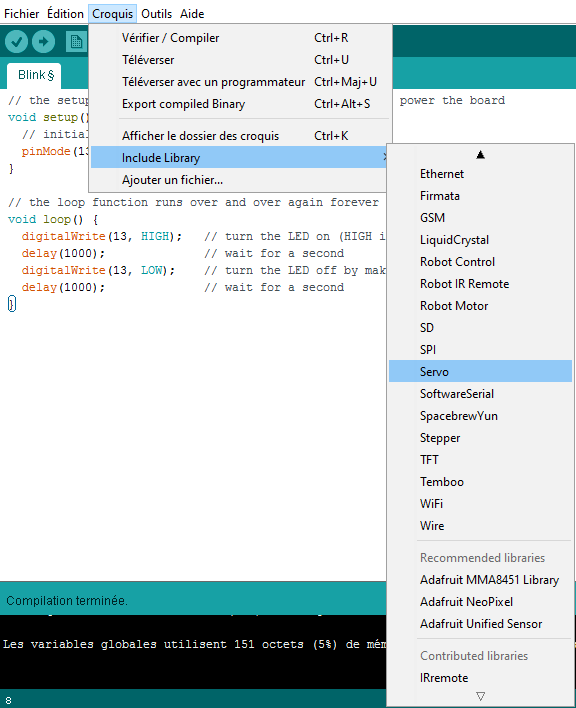
\includegraphics[scale=0.6]{rajouterlib.png}
    \caption{Import d'une bibliothèque}
    \label{fig:my_label}
\end{figure}

\bigskip
Il est également possible d’ajouter des bibliothèques non présentes de base. Pour ce faire, il faut tout d'abord télécharger cette dernière (format .zip). Après l'avoir décompressée, on obtient un dossier qu'il suffit de placer dans librairies du répértoire Arduino.

\bigskip
[Une bibliothèque possède en général des programmes d'exemples qui vous permettent d'illustrer son utilisation].

%----------------------------------------------------------------------------------------
%	REFERENCE LIST
%----------------------------------------------------------------------------------------

\bigskip
\begin{thebibliography}{99} % Bibliography - this is intentionally simple in this template

\bibitem[Personnalisez vos montages Arduino, 2013]{montageArduino:2013dg}.G. Spanner

 \bibitem[Le grand livre d’Arduino]{LivreArduino:2013dg}.E. Bartmann 
\end{thebibliography}

%----------------------------------------------------------------------------------------


\end{document}
